%%%%%%%%%%%%%%%%%%%%%%%%%%%%%%%%%%%%%%%%%
% Beamer Presentation
% LaTeX Template
% Version 1.0 (10/11/12)
%
% This template has been downloaded from:
% http://www.LaTeXTemplates.com
%
% License:
% CC BY-NC-SA 3.0 (http://creativecommons.org/licenses/by-nc-sa/3.0/)
%
%%%%%%%%%%%%%%%%%%%%%%%%%%%%%%%%%%%%%%%%%

%----------------------------------------------------------------------------------------
%	PACKAGES AND THEMES
%----------------------------------------------------------------------------------------
\documentclass[10pt,aspectratio=43,mathserif,UTF8]{beamer}

\mode<presentation> {

% The Beamer class comes with a number of default slide themes
% which change the colors and layouts of slides. Below this is a list
% of all the themes, uncomment each in turn to see what they look like.

%\usetheme{default}
%\usetheme{AnnArbor}
%\usetheme{Antibes}
%\usetheme{Bergen}
%\usetheme{Berkeley}
\usetheme{Berlin}
%\usetheme{Boadilla}
%\usetheme{CambridgeUS}
%\usetheme{Copenhagen}
%\usetheme{Darmstadt}
%\usetheme{Dresden}
%\usetheme{Frankfurt}
%\usetheme{Goettingen}
%\usetheme{Hannover}
%\usetheme{Ilmenau}
%\usetheme{JuanLesPins}
%\usetheme{Luebeck}
%\usetheme{Madrid}
%\usetheme{Malmoe}
%\usetheme{Marburg}
%\usetheme{Montpellier}
%\usetheme{PaloAlto}
%\usetheme{Pittsburgh}
%\usetheme{Rochester}
%\usetheme{Singapore}
%\usetheme{Szeged}
%\usetheme{Warsaw}

% As well as themes, the Beamer class has a number of color themes
% for any slide theme. Uncomment each of these in turn to see how it
% changes the colors of your current slide theme.

%\usecolortheme{albatross}
%\usecolortheme{beaver}
%\usecolortheme{beetle}
%\usecolortheme{crane}
%\usecolortheme{dolphin}
%\usecolortheme{dove}
%\usecolortheme{fly}
%\usecolortheme{lily}
%\usecolortheme{orchid}
\usecolortheme{rose}
%\usecolortheme{seagull}
%\usecolortheme{seahorse}
%\usecolortheme{whale}
%\usecolortheme{wolverine}

\setbeamertemplate{footline} % To remove the footer line in all slides uncomment this line
%\setbeamertemplate{footline}[page number] % To replace the footer line in all slides with a simple slide count uncomment this line

\setbeamertemplate{navigation symbols}{} % To remove the navigation symbols from the bottom of all slides uncomment this line
}
\batchmode
\usepackage{graphicx} % Allows including images
\usepackage{booktabs} % Allows the use of \toprule, \midrule and \bottomrule in tables
\usepackage{animate}
\usepackage {subcaption}

%导入一些用到的宏包
\usepackage{amssymb}
\usepackage{amsthm}
\usepackage{amsmath}
\usepackage{amsfonts}
\usepackage[UTF8]{ctex}
\usepackage{setspace}
\usepackage{bm,enumerate,epsfig,bbm,calc,color,ifthen,capt-of,multimedia,hyperref}
\usepackage{multirow}
\usepackage{xcolor}
\usepackage{tikz}
\usetikzlibrary{arrows,shapes,chains}
\setstretch{1.05} 
\usefonttheme[onlymath]{serif}


%----------------------------------------------------------------------------------------
%	TITLE PAGE
%----------------------------------------------------------------------------------------

\title{Hartree-Fock自洽场迭代收敛算法实现与测试
} % The short title appears at the bottom of every slide, the full title is only on the title page

\author{答辩人: 张凌志 \newline \newline 指导教师: 马海波} % Your name
\institute % Your institution as it will appear on the bottom of every slide, may be shorthand to save space
{
南京大学化学化工学院 \\ % Your institution for the title page
\medskip
%\textit{171840719@smail.nju.edu.cn} % Your email address
}
\date{\today} % Date, can be changed to a custom date

\begin{document}
\begin{frame}
\titlepage % Print the title page as the first slide
\end{frame}

\begin{frame}
\frametitle{目录} % Table of contents slide, comment this block out to remove it
\tableofcontents % Throughout your presentation, if you choose to use \section{} and \subsection{} commands, these will automatically be printed on this slide as an overview of your presentation
\end{frame}

%----------------------------------------------------------------------------------------
%	PRESENTATION SLIDES
%----------------------------------------------------------------------------------------

%------------------------------------------------
\section{研究背景与意义} % Sections can be created in order to organize your presentation into discrete blocks, all sections and subsections are automatically printed in the table of contents as an overview of the talk
%------------------------------------------------



%------------------------------------------------
\subsection{从多电子哈密顿到单电子平均场近似}
\begin{frame}
	\frametitle{从多电子哈密顿到单电子平均场近似}
	%薛定谔方程
	%\begin{align}
	%	\hat{H}\Psi = i\hbar \frac{\partial \Psi}{\partial t}
	%\end{align}
	多电子哈密顿量
	\begin{align}
		\hat{H}  = \sum_{i=1}^{n} -\frac{1}{2} \nabla_i ^ {2} - 
		\sum_{i=1}^{n}\sum_{a=1}^{N_a} \frac{Z_a}{r_{ai}} + \sum_{a>b} \frac{Z_a Z_b}{r_{ab}} + 
		\sum_{i>j} \frac{1}{r_{ij}}
	\end{align}

	平均场近似:将多体问题转变为单体问题,求解多电子哈密顿量转变为求解单电子算符。

	\begin{figure}[ht!]
		\centering
		\begin{subfigure}{0.4\linewidth}
			\centering
			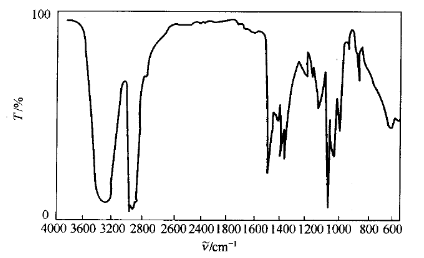
\includegraphics[height=3cm]{figure/HF/ultra.png}
			\subcaption{异丁醇红外光谱图}
			\label{fig:light}
		\end{subfigure}
		\begin{subfigure}{0.4\linewidth}
			\centering
			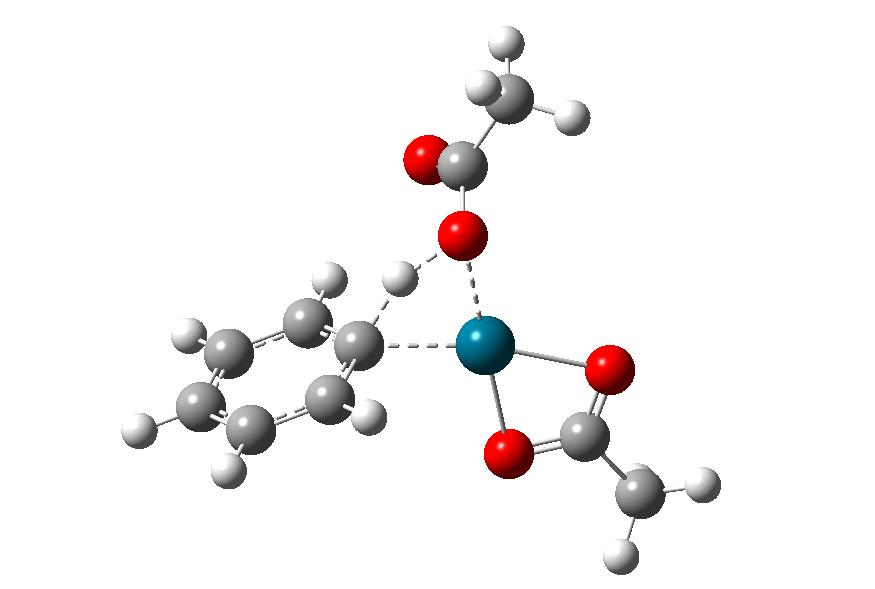
\includegraphics[height=3cm]{figure/HF/ts.jpg}
			\subcaption{过渡金属催化反应过渡态}
			\label{fig:ts}
		\end{subfigure}
		\label{fig:ref}
	\end{figure}

\end{frame}

%------------------------------------------------
\subsection{Hartree-Fock计算}
\begin{frame}
\frametitle{Hartree-Fock计算}
Hartree-Fock-Roothaan方程(HFR方程)
\begin{equation}
	FC=SCE
\end{equation}

\begin{figure}[htbp]
	\centering
	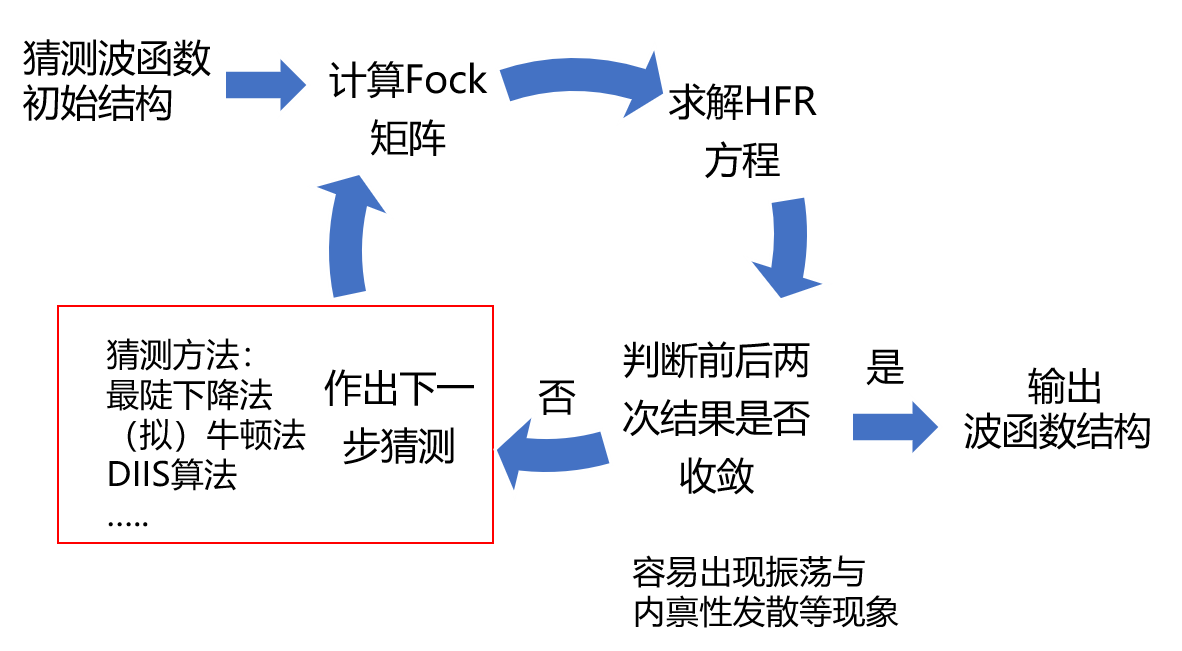
\includegraphics[width=0.7\textwidth]{figure/HF/HF_process3.png}
\end{figure}
\end{frame}


%------------------------------------------------
\section{研究内容}
%------------------------------------------------
\begin{frame}
\frametitle{研究内容}
	\begin{itemize}
		\item 将DIIS类算法应用在Hartree-Fock计算中;\\
		DIIS算法、EDIIS算法与C$^2$DIIS算法
		\item 将直接最小化算法应用在Hartree-Fock计算p中;\\
		梯度下降法、拟牛顿法、RFO算法、RS-RFO算法与QN/DIIS算法
		\item 确定一种算法的组合策略以应对大多数体系的Hartree-Fock计算。
	\end{itemize}

\end{frame}


%------------------------------------------------
\subsection{DIIS类算法}
\begin{frame}
	\frametitle{DIIS(Direct Inversion in Iterative Space)类算法}
	利用多步的信息来调整下一步迭代的输入,实现了DIIS算法、C$^2$DIIS算法与EDIIS算法。
	
	\begin{columns}
		\column{.45\textwidth} % Left column and width
		\begin{figure}  
			\scriptsize  
			\tikzstyle{startstop} = [rectangle,rounded corners, minimum width=3cm,minimum height=1cm,text centered, draw=black,fill=red!30]
			\tikzstyle{format}=[rectangle,draw,thin,fill=white]  
			%定义语句块的颜色,形状和边
			\tikzstyle{test}=[diamond,aspect=2,draw,thin]  
			%定义条件块的形状,颜色
			\tikzstyle{point}=[coordinate,on grid,]  
			%像素点,用于连接转移线
			\begin{tikzpicture}%[node distance=10mm,auto,>=latex',thin,start chain=going below,every join/.style={norm},] 
			%start chain=going below指明了流程图的默认方向,node distance=8mm则指明了默认的node距离。这些可以在定义node的时候更改,比如说 
			%\node[point,right of=n3,node distance=10mm] (p0){};  
			%这里声明了node p0,它在node n3 的右边,距离是10mm。
			\node[format] (start){输入前n步信息};
			\node[format,below of=start,node distance=7mm] (define){设定新密度矩阵 \newline $D^*=\sum_{i=1}^n c_iD_i$};
			\node[format,below of=define,node distance=7mm] (define1){设定新误差向量 \newline $e^*=\sum_{i=1}^n c_ie_i$};
			\node[format,below of=define1,node distance=7mm] (PCFinit){根据不同算法优化 \newline 得到系数$\{c_i\}$};
			\node[format,below of=PCFinit,node distance=7mm] (DS18init){将$D^*$作为 \newline 下一步迭代输入};
			%\node[format] (n0) at(4,4){A}; 直接指定位置 
			%定义完node之后进行连线,
			%\draw[->] (n0.south) -- (n1); 带箭头实线
			%\draw[-] (n0.south) -- (n1); 不带箭头实线
			%\draw[<->] (n0.south) -- (n1.north);   双箭头
			%\draw[<-,dashed] (n1.south) -- (n2.north); 带箭头虚线 
			%\draw[<-] (n0.south) to node{Yes} (n1.north);  带字,字在箭头方向右边
			%\draw[->] (n1.north) to node{Yes} (n0.south);  带字,字在箭头方向左边
			%\draw[->] (n1.north) to[out=60,in=300] node{Yes} (n0.south);  曲线
			%\draw[->,draw=red](n2)--(n1);  带颜色的线
			\draw[->] (start)--(define);
			\draw[->] (define)--(define1);
			\draw[->] (define1)--(PCFinit);
			\draw[->](PCFinit)--(DS18init);
			\end{tikzpicture}  
		\end{figure}  
		
		\column{.5\textwidth} % Right column and width
		\textbf{不同点}
		\begin{enumerate}
		\item DIIS算法在$\sum_{i=1}^n c_i = 1$约束下最小化$\Vert e \Vert$
		\item C$^2$DIIS算法在$\sum_{i=1}^n c_i^2 = 1$约束下最小化$\Vert e \Vert$
		\item EDIIS算法在寻找使得能量泛函最低的内插值
		\end{enumerate}
		
		
	\end{columns}

\end{frame}



%------------------------------------------------
\begin{frame}
	\frametitle{EDIIS算法与DIIS算法结果比较}
	\begin{columns}[c]
		\column{.5\textwidth}
		\begin{figure}[htbp]
			\centering
			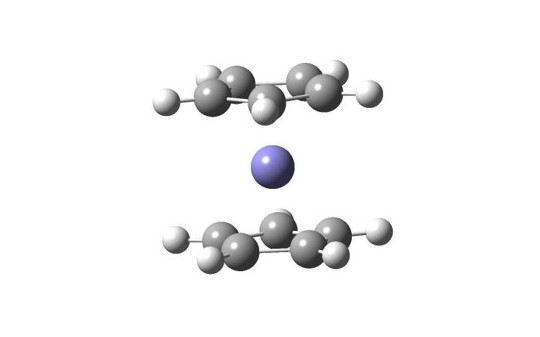
\includegraphics[height=2cm]{figure/ferrocene/ferrocene2.jpg}
		\end{figure}

		\column{.5\textwidth}
		二茂铁\\
		RHF/6-31G基组
	\end{columns}

	\begin{figure}[ht!]
		\centering
		\begin{minipage}{0.4\linewidth}
			\centering
			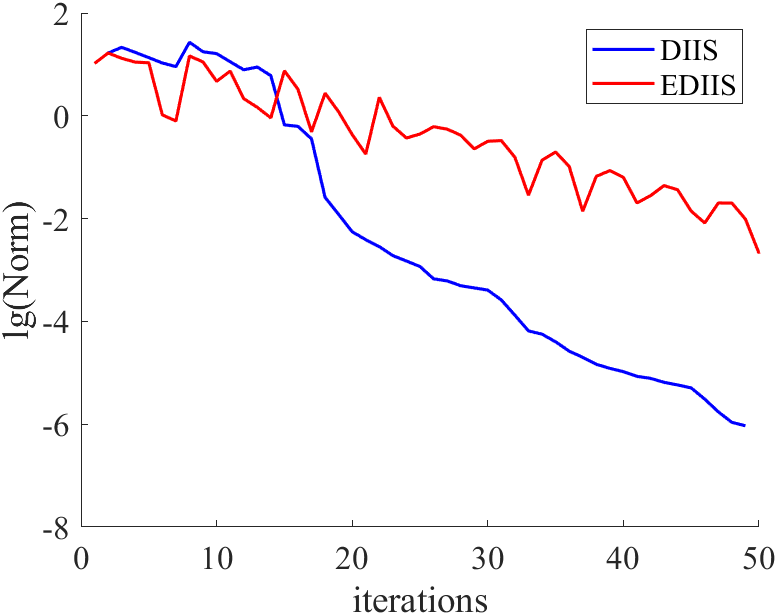
\includegraphics[height=3cm]{figure/ferrocene/logNorm4.png}
			\subcaption{梯度的模变化趋势}
			\label{fig:ferrocene:lognorm}
		\end{minipage}
		\begin{minipage}{0.4\linewidth}
			\centering
			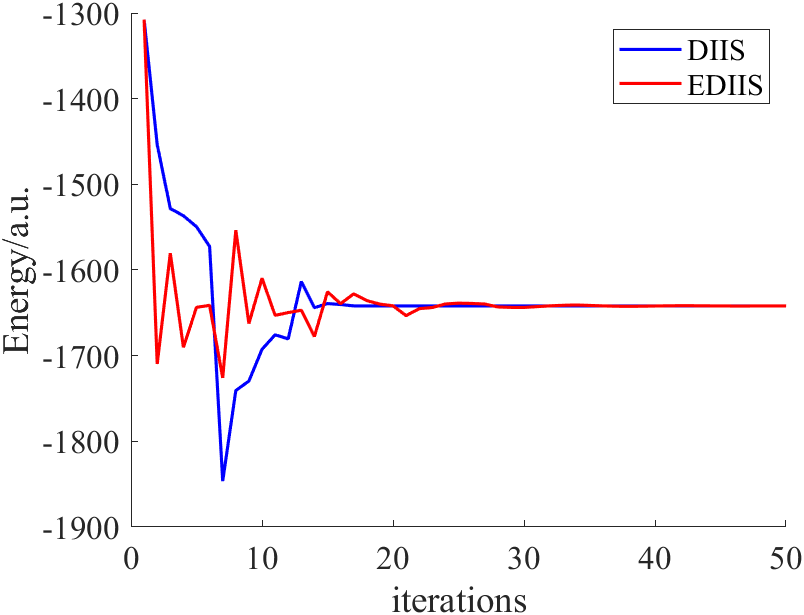
\includegraphics[height=3cm]{figure/ferrocene/E4.png}
			\subcaption{能量变化趋势}
			\label{fig:ferrocene:E}
		\end{minipage}
		\label{fig:ferrocene}
	\end{figure}
	\centerline{EDIIS算法的使用可以在初期快速降低迭代过程中的能量。}
\end{frame}

%------------------------------------------------
\begin{frame}
	\frametitle{EDIIS算法对收敛结果的影响}
	HFR方程存在多个自洽解,往往我们需要能量最低的自洽解。\\
	
	\begin{columns}[c]
		\column{.5\textwidth}
		\begin{figure}[htbp]
			\centering
			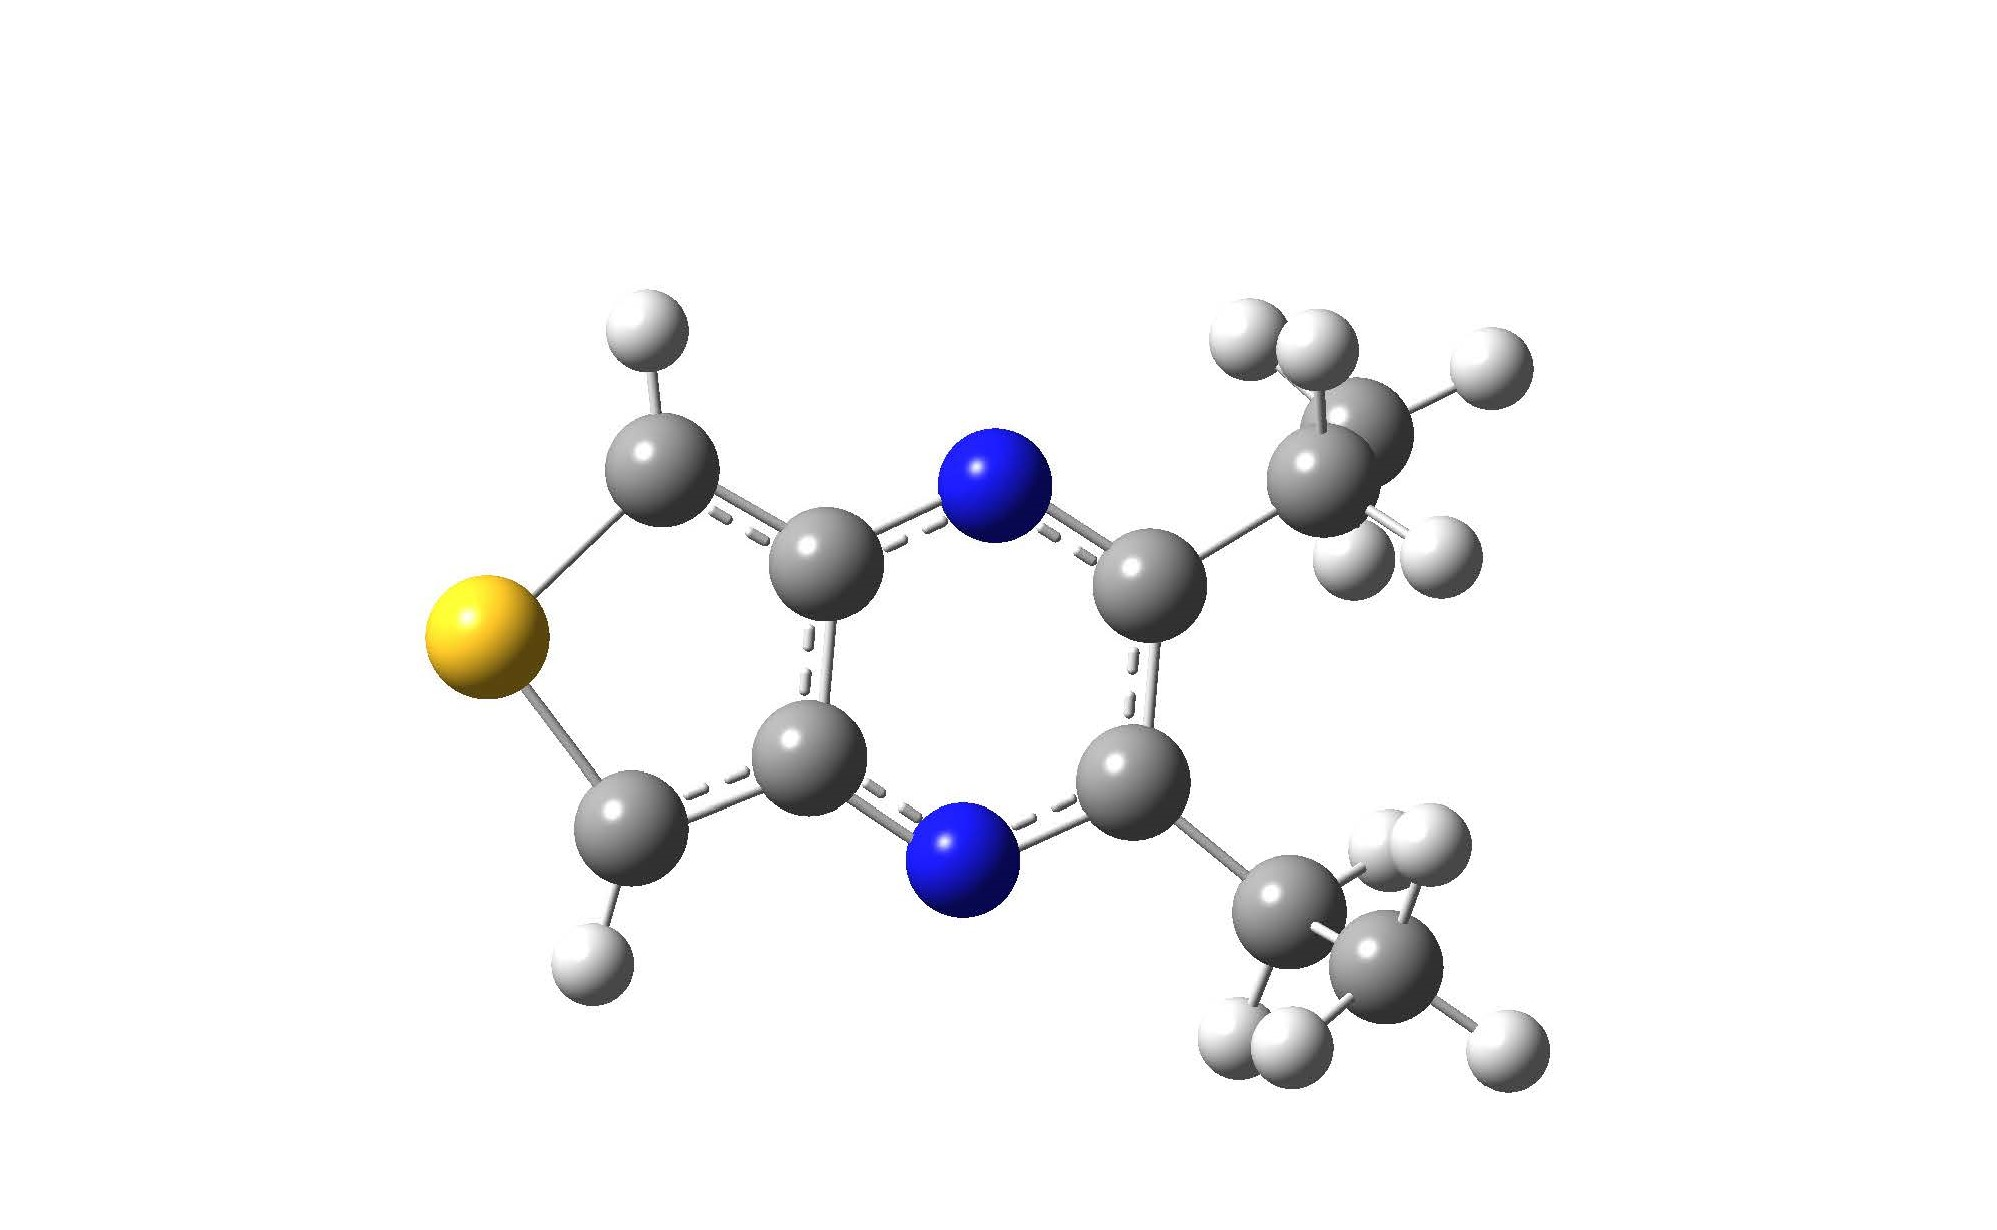
\includegraphics[height=2.2cm]{figure/AA4/AA42.jpg}
		\end{figure}

		\column{.5\textwidth}
		2,3-二乙基噻吩[3,4-B]吡嗪\\
		UHF/6-31G基组
	\end{columns}

	\begin{table}[htbp]
		%\centerline{2,3-二乙基噻吩[3,4-B]吡嗪的UHF计算结果。}
		\caption{2,3-二乙基噻吩[3,4-B]吡嗪的UHF计算结果。}\label{table:AA4}
		\setlength{\belowcaptionskip}{7pt}
		\centering
		\begin{tabular}{l l l}
			\toprule
			\textbf{算法}		&\textbf{能量/(a.u.)}	&\textbf{迭代圈数}\\
			\midrule
			DIIS				& -891.580787		&57\\
			EDIIS				& -891.734354		&538\\
			EDIIS+DIIS			& -891.734354		&90\\
			\bottomrule
		\end{tabular}
		\vspace{0.2cm}
	\end{table}
	\centerline{EDIIS算法可以辅助程序收敛到能量更低的解。}
\end{frame}

%------------------------------------------------
\begin{frame}
	\frametitle{DIIS算法与C$^2$DIIS算法结果比较}
	C$^2$DIIS算法主要应对DIIS算法中存在奇点的问题\\
	\begin{columns}[c]
		\column{.5\textwidth}
		\begin{figure}[htbp]
			\centering
			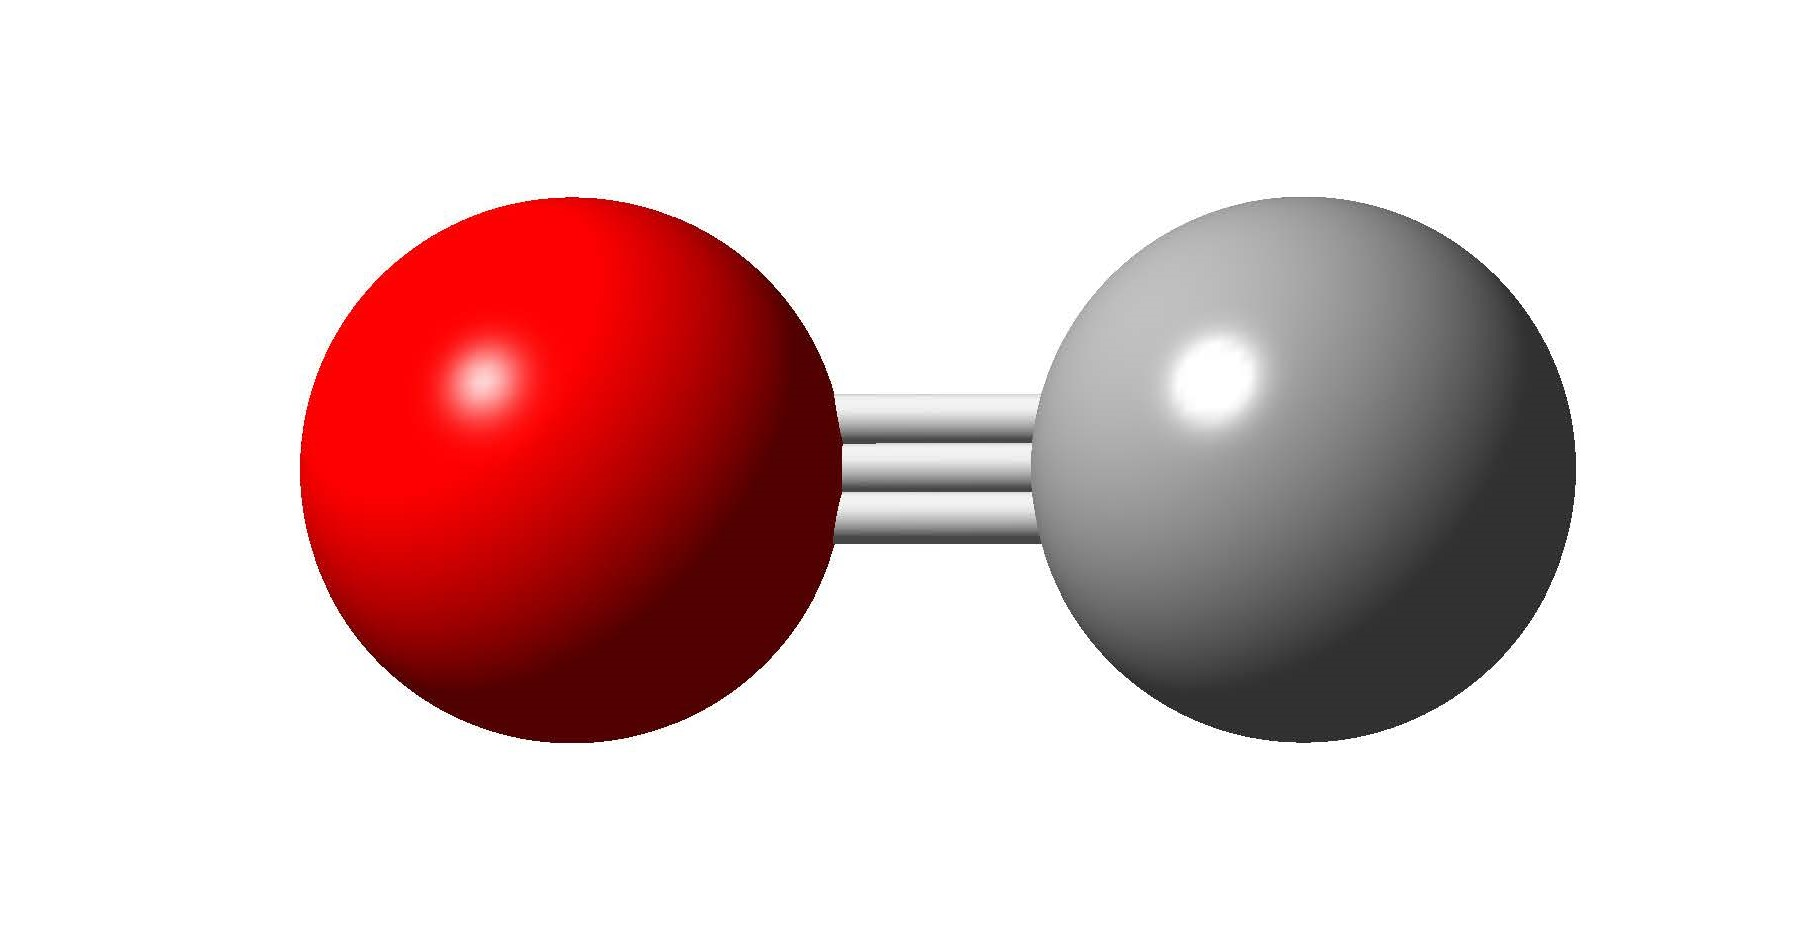
\includegraphics[height=1cm]{figure/co/CO2.jpg}
		\end{figure}

		\column{.5\textwidth}
		一氧化碳\\
		UHF/6-31G基组
	\end{columns}
	\begin{figure}[ht!]
		\centering
		\begin{minipage}{0.4\linewidth}
			\centering
			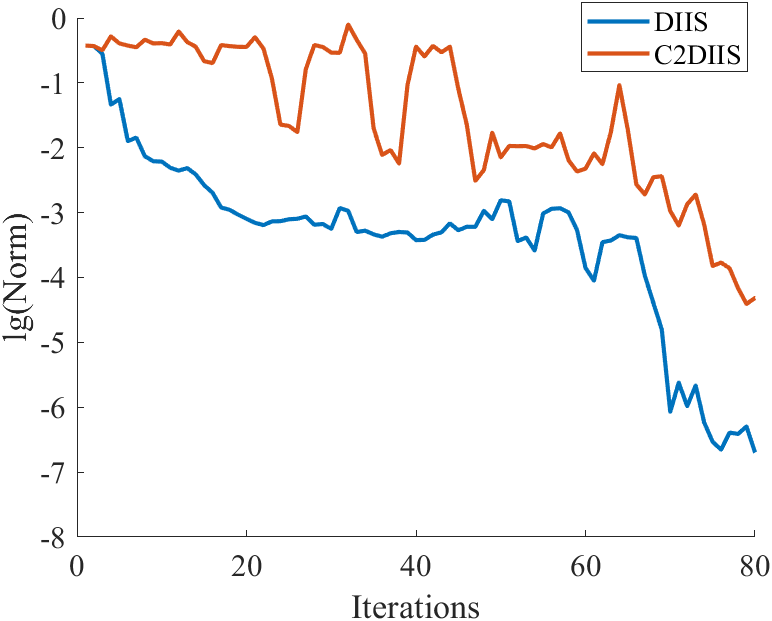
\includegraphics[height=3cm]{figure/co/LOG3.png}
			\subcaption{梯度的模变化趋势}
			\label{fig:co:lognorm}
		\end{minipage}
		\begin{minipage}{0.4\linewidth}
			\centering
			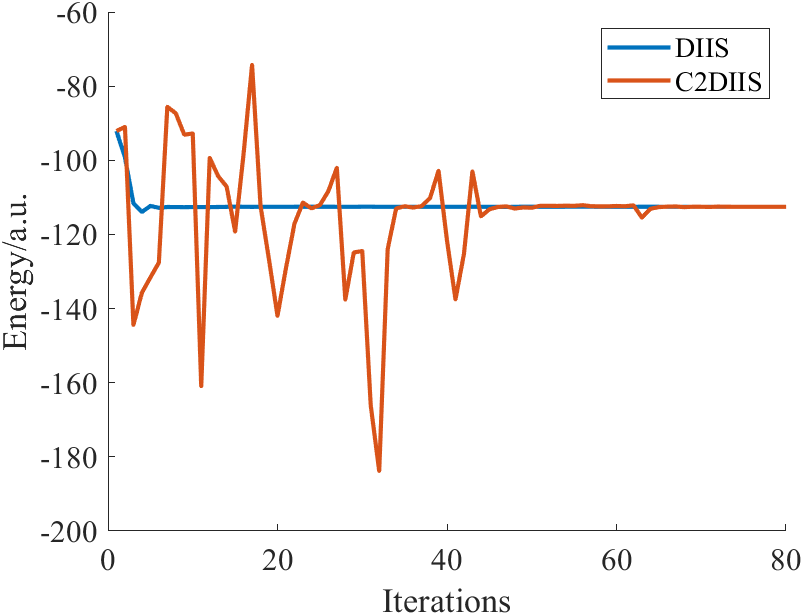
\includegraphics[height=3cm]{figure/co/E4.png}
			\subcaption{能量变化趋势}
			\label{fig:co:E}
		\end{minipage}
		\label{fig:co}
	\end{figure}
	\centerline{DIIS算法表现优异可以很快收敛,C$^2$DIIS算法性能逊于DIIS算法。}
\end{frame}


%------------------------------------------------
\subsection{直接最小化算法}
\begin{frame}
	\frametitle{直接最小化算法}
	Hartree-Fock方法的本质是在归一化条件下优化Hartree-Fock基态能量
	\begin{equation}
	E_{0}=\text{min}\left \{ E_{\text{HF}}(C)  | C^TSC=I   \right \}
	\end{equation}
	可以直接优化参数求函数最小值,计算流程如下

	\begin{figure}[htbp]
		\centering
		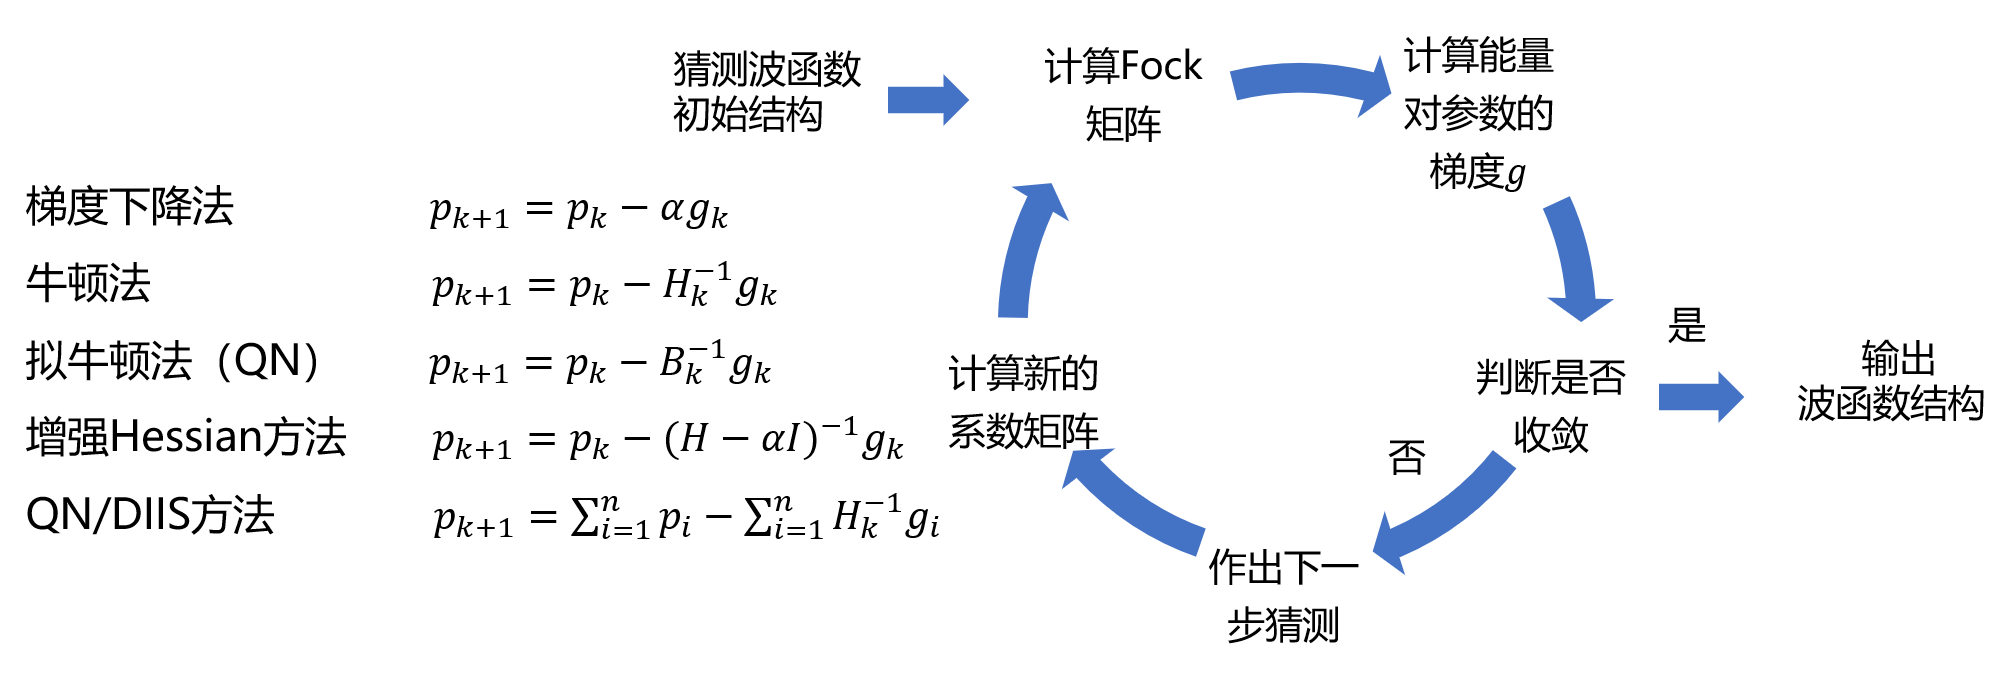
\includegraphics[width=1.0\textwidth]{figure/HF/QN5.png}
	\end{figure}
	%\begin{columns}[c] % The "c" option specifies centered vertical alignment while the "t" option is used for top vertical alignment

		%\column{.5\textwidth} % Left column and width
		%\begin{figure}[htbp]
		%	\centering
		%	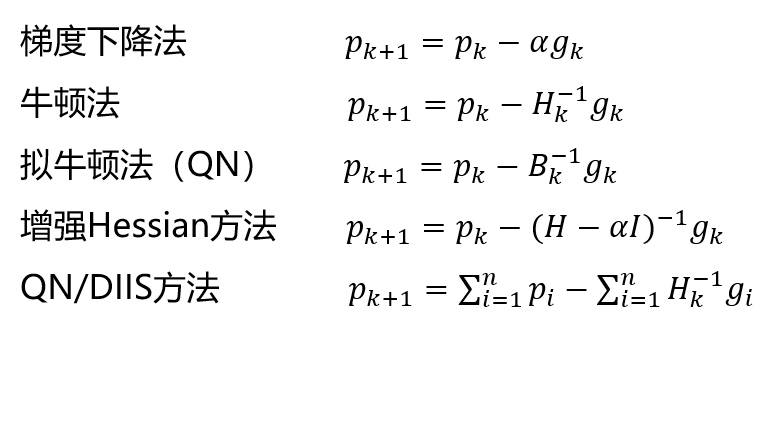
\includegraphics[width=1\textwidth]{figure/HF/QN4.png}
		%\end{figure}
		%\textbf{算法}
		%\begin{enumerate}
		%\item 梯度下降法		$p_{k+1}=p_{k} - \alpha g_k$
		%\item 牛顿法			$p_{k+1}=p_{k} - H_k^{-1} g_k$
		%\item 拟牛顿法(QN)	$p_{k+1}=p_{k} - B_k^{-1} g_k$
		%\item 增强Hessian方法	$p_{k+1}=p_{k} - (H -\lambda I)^{-1} g_k$
		%\item QN/DIIS方法		$ p_{k+1}=\sum_{i=1}^n p_{i} - \sum_{i=1}^n H_k^{-1} g_i $
		%\end{enumerate}
		
		%\column{.5\textwidth} % Right column and width
		%\begin{figure}[htbp]
			%\centering
			%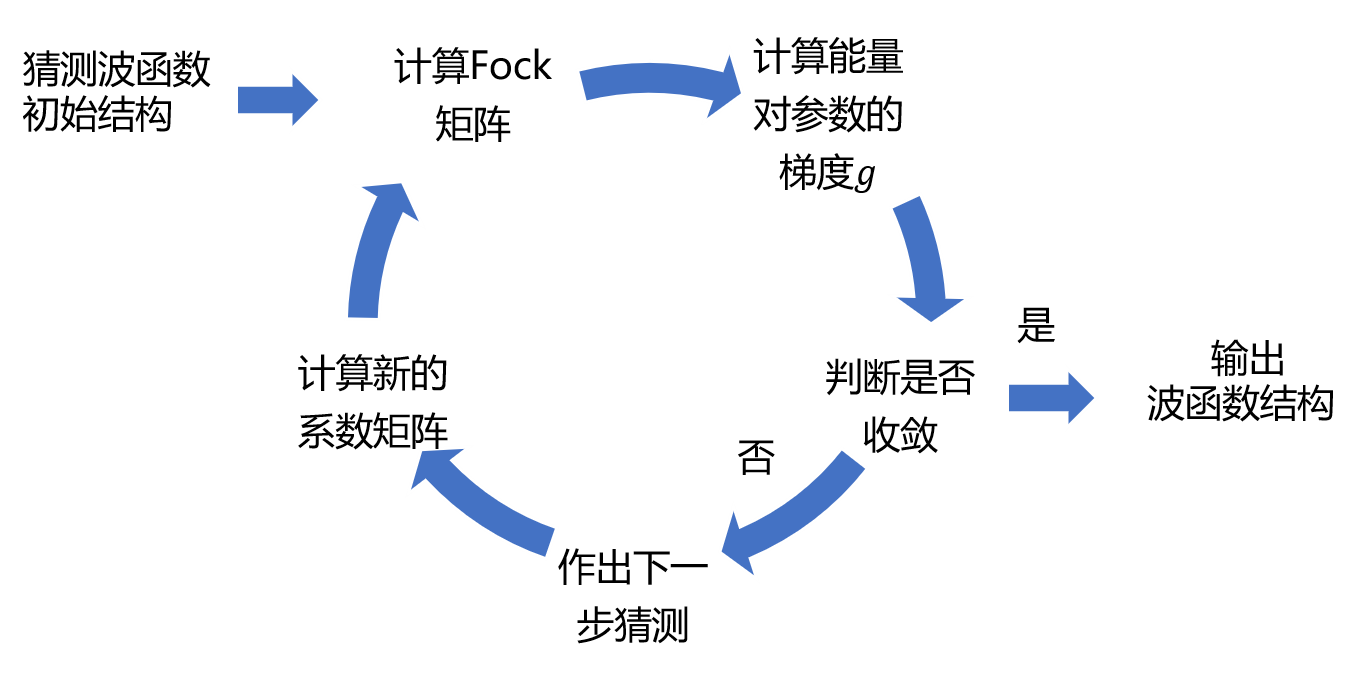
\includegraphics[width=1\textwidth]{figure/HF/QN3.png}
		%\end{figure}
	%end{columns}
	%$p_k$代表第$k$步的参数
	%$g_k$代表第$k$步的梯度向量\\
	%$H_k$代表第$k$步的Hessian矩阵\\
	%$B_k$代表第$k$步的Hessian矩阵的近似。

	%$g_k$代表第$k$步的梯度向量\\
	%$H_k$代表第$k$步的Hessian矩阵\\
	%$B_k$代表第$k$步的Hessian矩阵的近似。
	
\end{frame}



%------------------------------------------------
\begin{frame}
	\frametitle{结果比较}
	\begin{columns}[c]
		\column{.5\textwidth}
		\begin{figure}[htbp]
			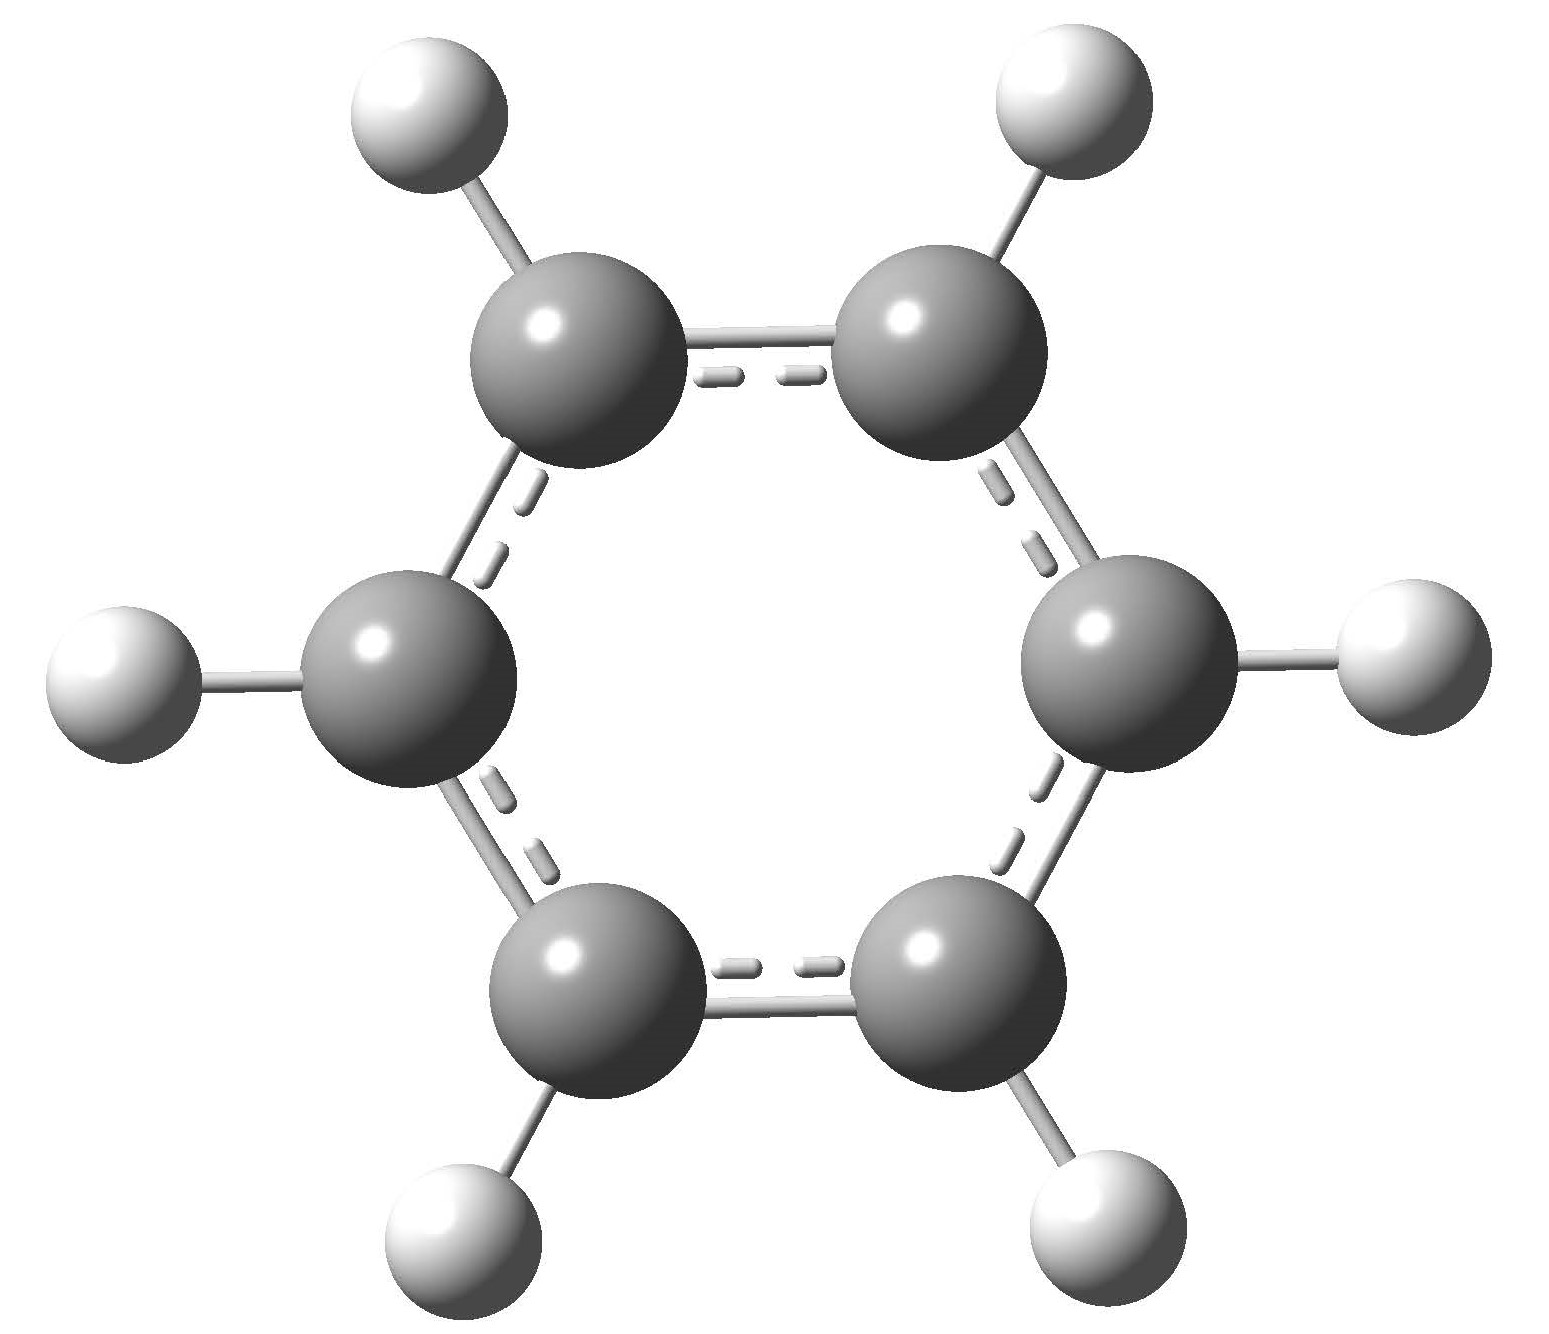
\includegraphics[height=1.7cm]{figure/benzene/benzene2.jpg}
		\end{figure}

		\column{.5\textwidth}
		苯分子\\
		UHF/6-31G基组
		
	\end{columns}
	
	\begin{figure}[ht!]
		\centering
		\begin{minipage}{0.4\linewidth}
			\centering
			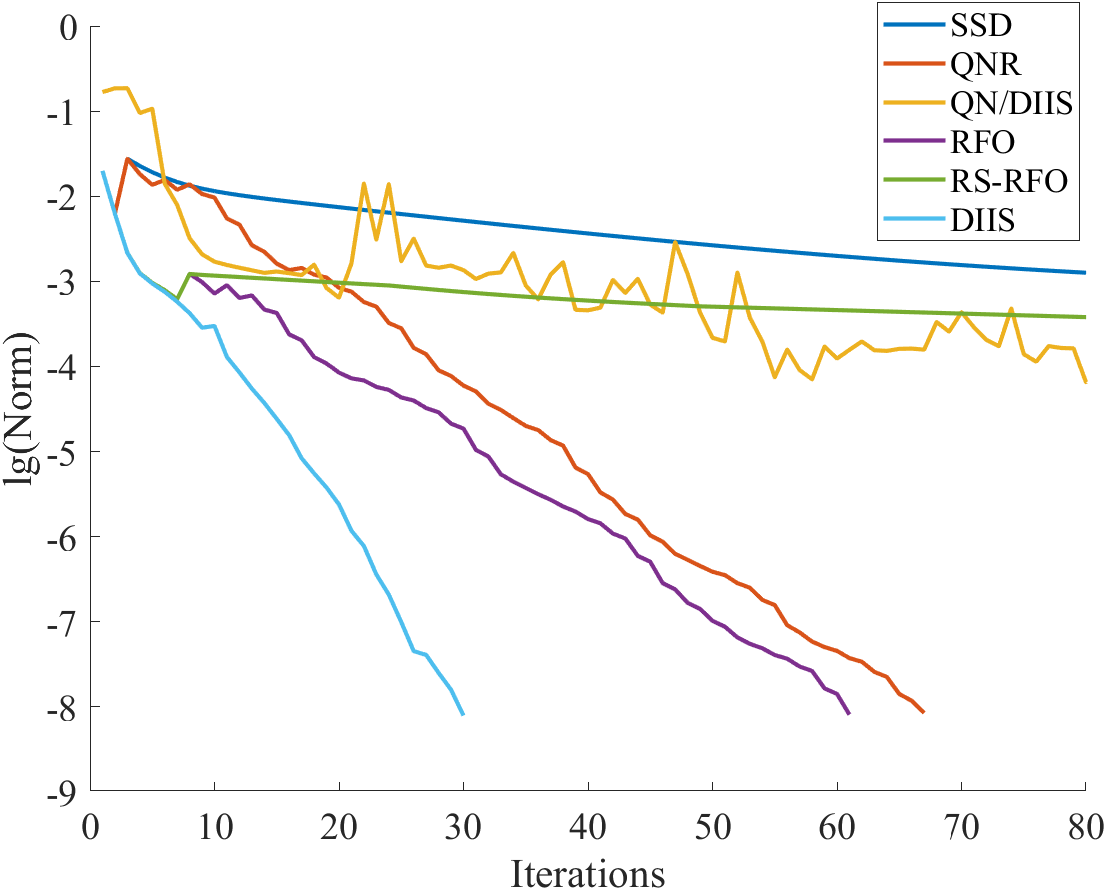
\includegraphics[height=3cm]{figure/benzene/NORM7.png}
			\subcaption{梯度的模变化趋势}
			\label{fig:benzene:lognorm}
		\end{minipage}
		\begin{minipage}{0.4\linewidth}
			\centering
			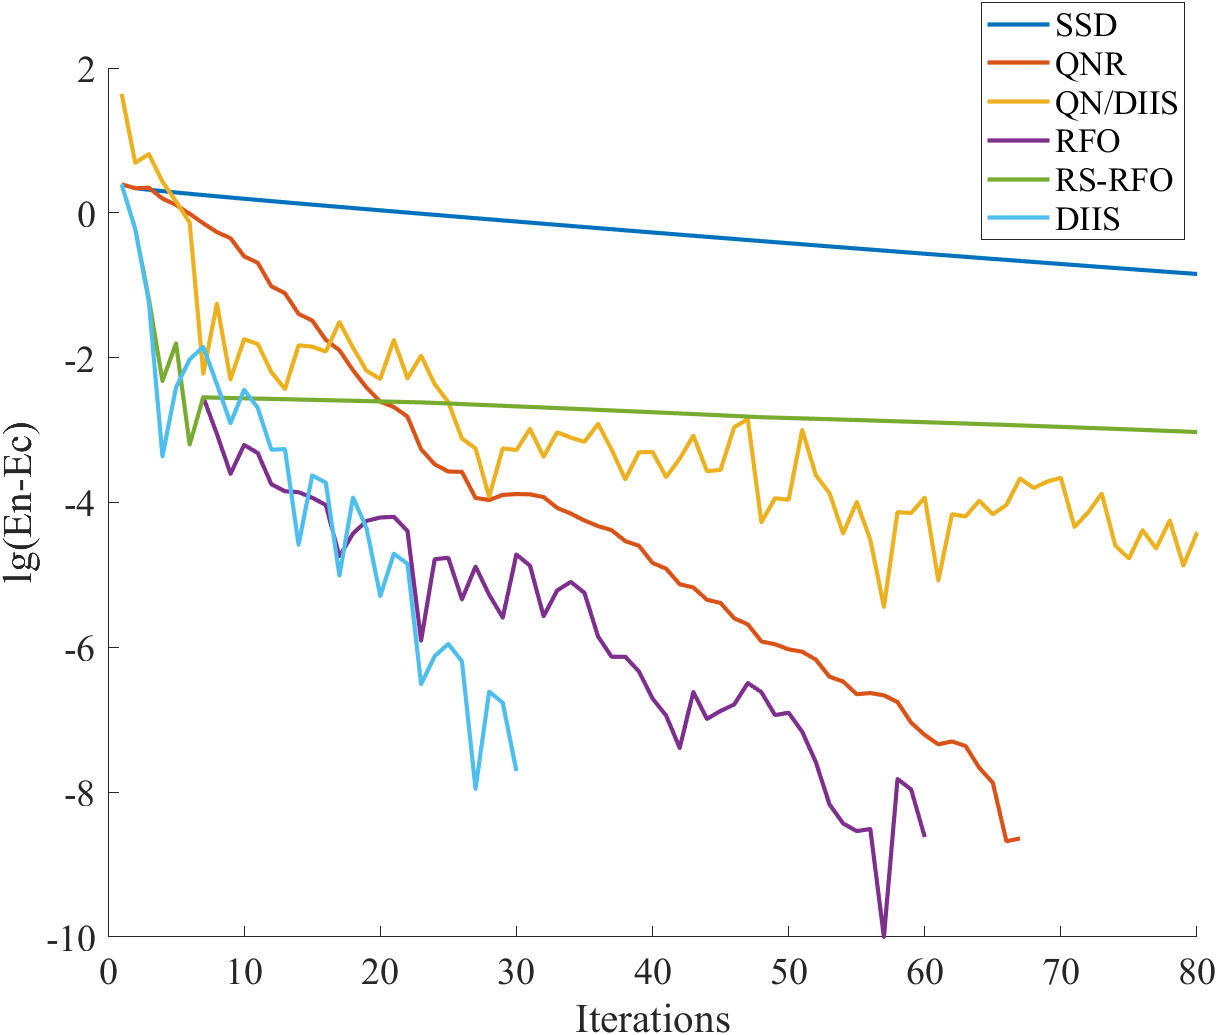
\includegraphics[height=3cm]{figure/benzene/E8.png}
			\subcaption{能量变化趋势}
			\label{fig:benzene:E1}
		\end{minipage}
	\end{figure}
	拟牛顿法与RFO算法的表现相对良好,SSD算法收敛速度较慢,QN/DIIS算法振荡明显,RS-RFO算法收敛失败。
\end{frame}
%------------------------------------------------
\subsection{组合算法}
\begin{frame}
	\frametitle{组合算法}
	在实际计算,单个算法的效果存在局限性——EDIIS算法收敛速度太慢,DIIS算法有时候易收敛到局域极小值。\\
	程序采用EDIIS算法与DIIS算法的组合,组合方式如下:
	
	\begin{figure}[htbp]
		\centering
		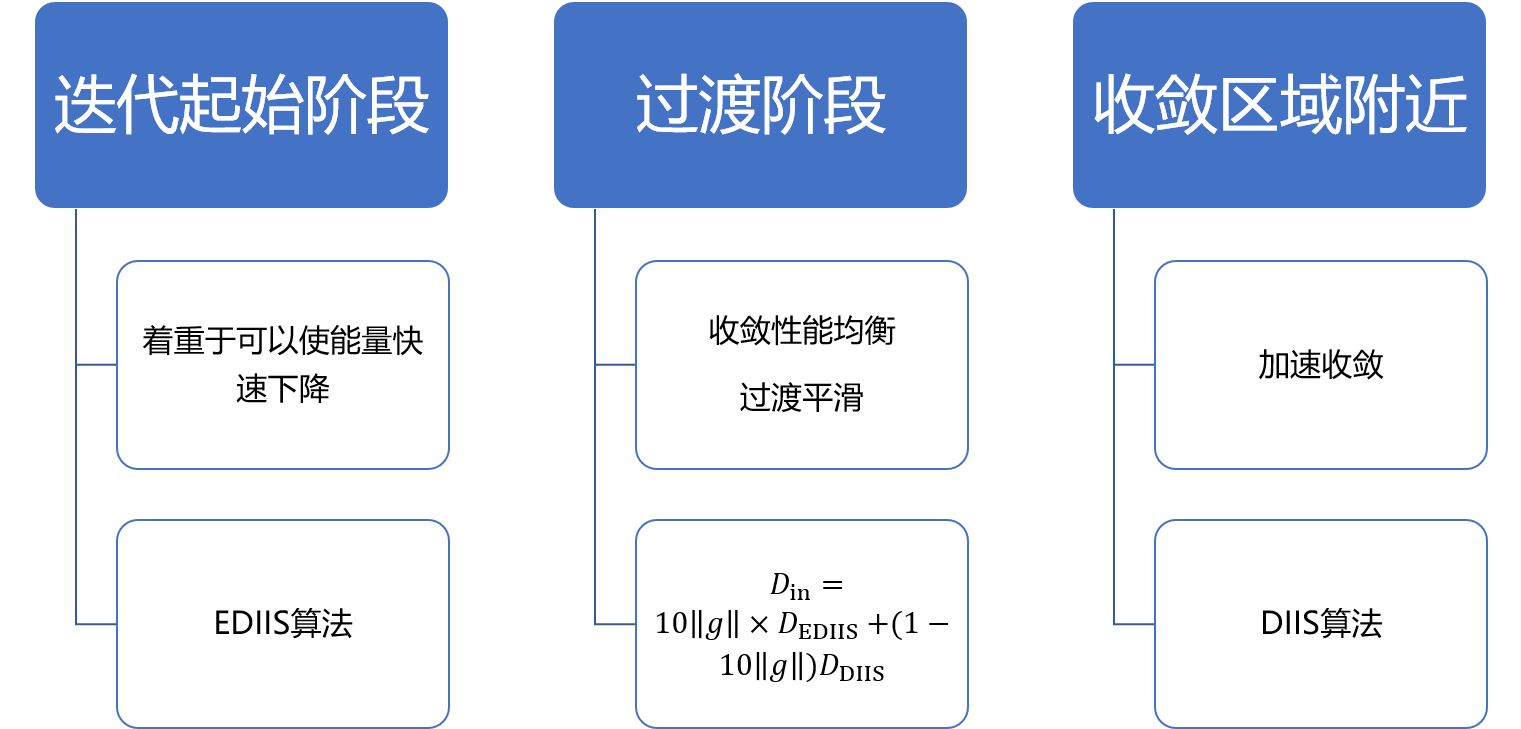
\includegraphics[width=0.7\textwidth]{figure/HF/idea3.png}
	\end{figure}
	
	%$\Vert g \Vert$为计算中能量对于轨道旋转矩阵元素的梯度的模。

	
\end{frame}


%------------------------------------------------
\begin{frame}
	\frametitle{结果比较}
	\begin{columns}[c]
		\column{.5\textwidth}
		\begin{figure}[htbp]
			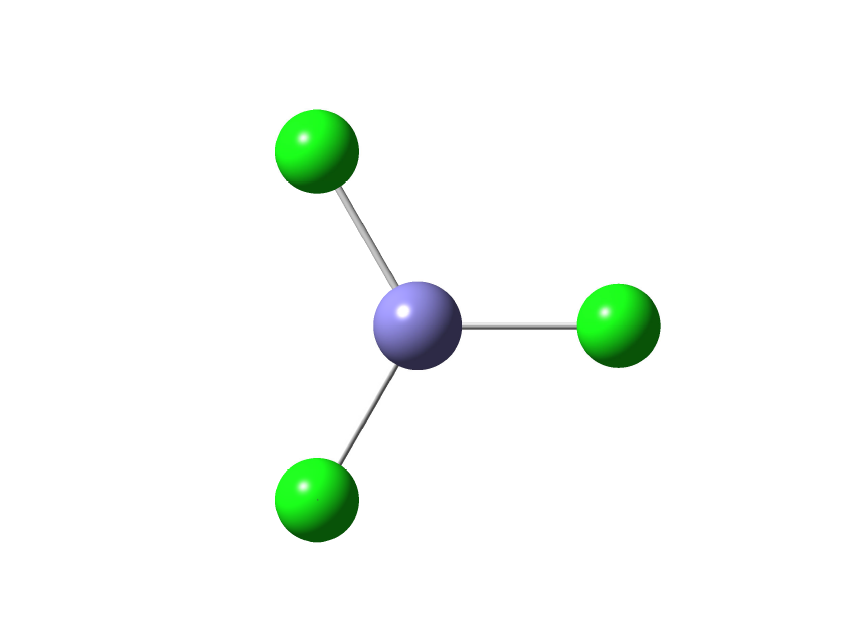
\includegraphics[height=2cm]{figure/FeCl3/FeCl32.png}
		\end{figure}

		\column{.5\textwidth}
		三氯化铁\\
		UHF/铁原子cc-pvdz基组,氯原子6-31G基组
	\end{columns}
	\begin{figure}[ht!]
		\centering
		\begin{minipage}{0.4\linewidth}
			\centering
			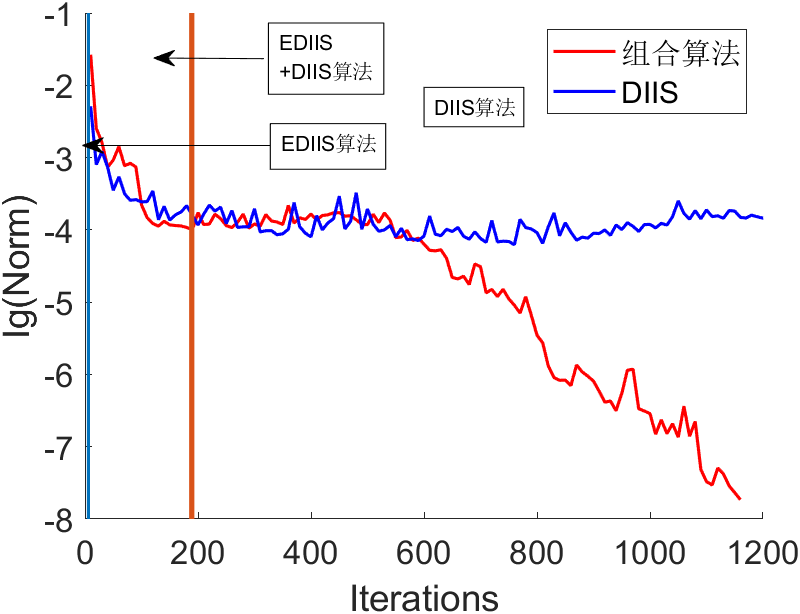
\includegraphics[height=3cm]{figure/FeCl3/NORM4.png}
			\subcaption{梯度的模变化趋势}
			\label{fig:FeCl3:E}
		\end{minipage}
		\begin{minipage}{0.4\linewidth}
			\centering
			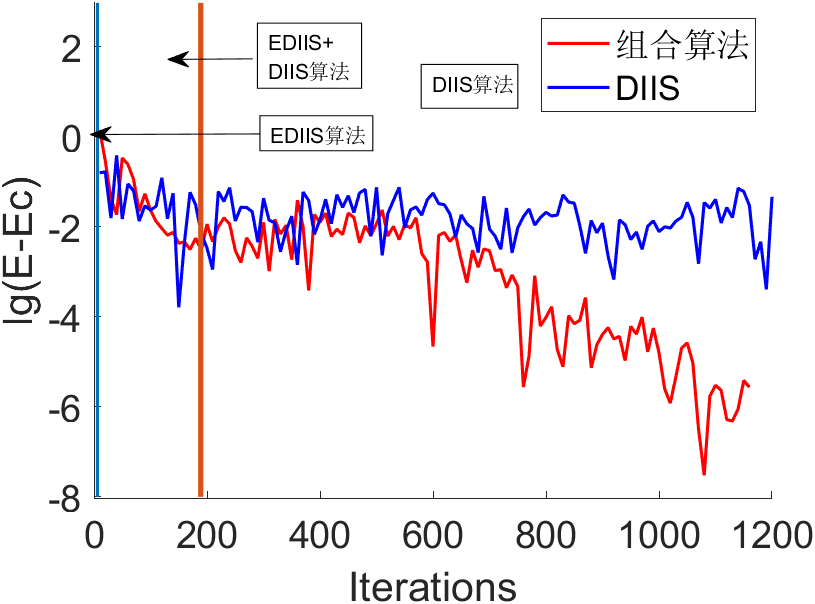
\includegraphics[height=3cm]{figure/FeCl3/E5.png}
			\subcaption{收敛区域能量变化趋势}
			\label{fig:FeCl3:FD}
		\end{minipage}
	\end{figure}
	前期使用EDIIS算法可以有效抑制收敛区域的振荡,辅助收敛。
\end{frame}

%----------------------------------------------------------------------------------------
\section{研究总结与展望}
%----------------------------------------------------------------------------------------

\begin{frame}
	\frametitle{研究总结与展望}
	\textbf{总结}
	\begin{itemize}
		\item[1)]
		 实现了DIIS类算法与直接最小化算法,并对其进行测试;
		\item[2)] 
		 设计出一种组合算法,可以对大多数体系进行Hartree-Fock计算,包括含过渡金属的小分子体系。
	\end{itemize}
	
	\begin{columns}[c]
		
		\column{.6\textwidth} % Left column and width
		\textbf{展望}
		\begin{enumerate}
			\item [1)]
			EDIIS算法中参数优化算法需要进一步调整;
			\item [2)]
			各种算法之间的切换仍需进一步调整优化;
			\item [3)]
			进一步优化整体算法以计算含过渡金属的大分子体系。
		\end{enumerate}
	
		\column{.4\textwidth} % right column and width
		\begin{figure}[htbp]
			\centering
			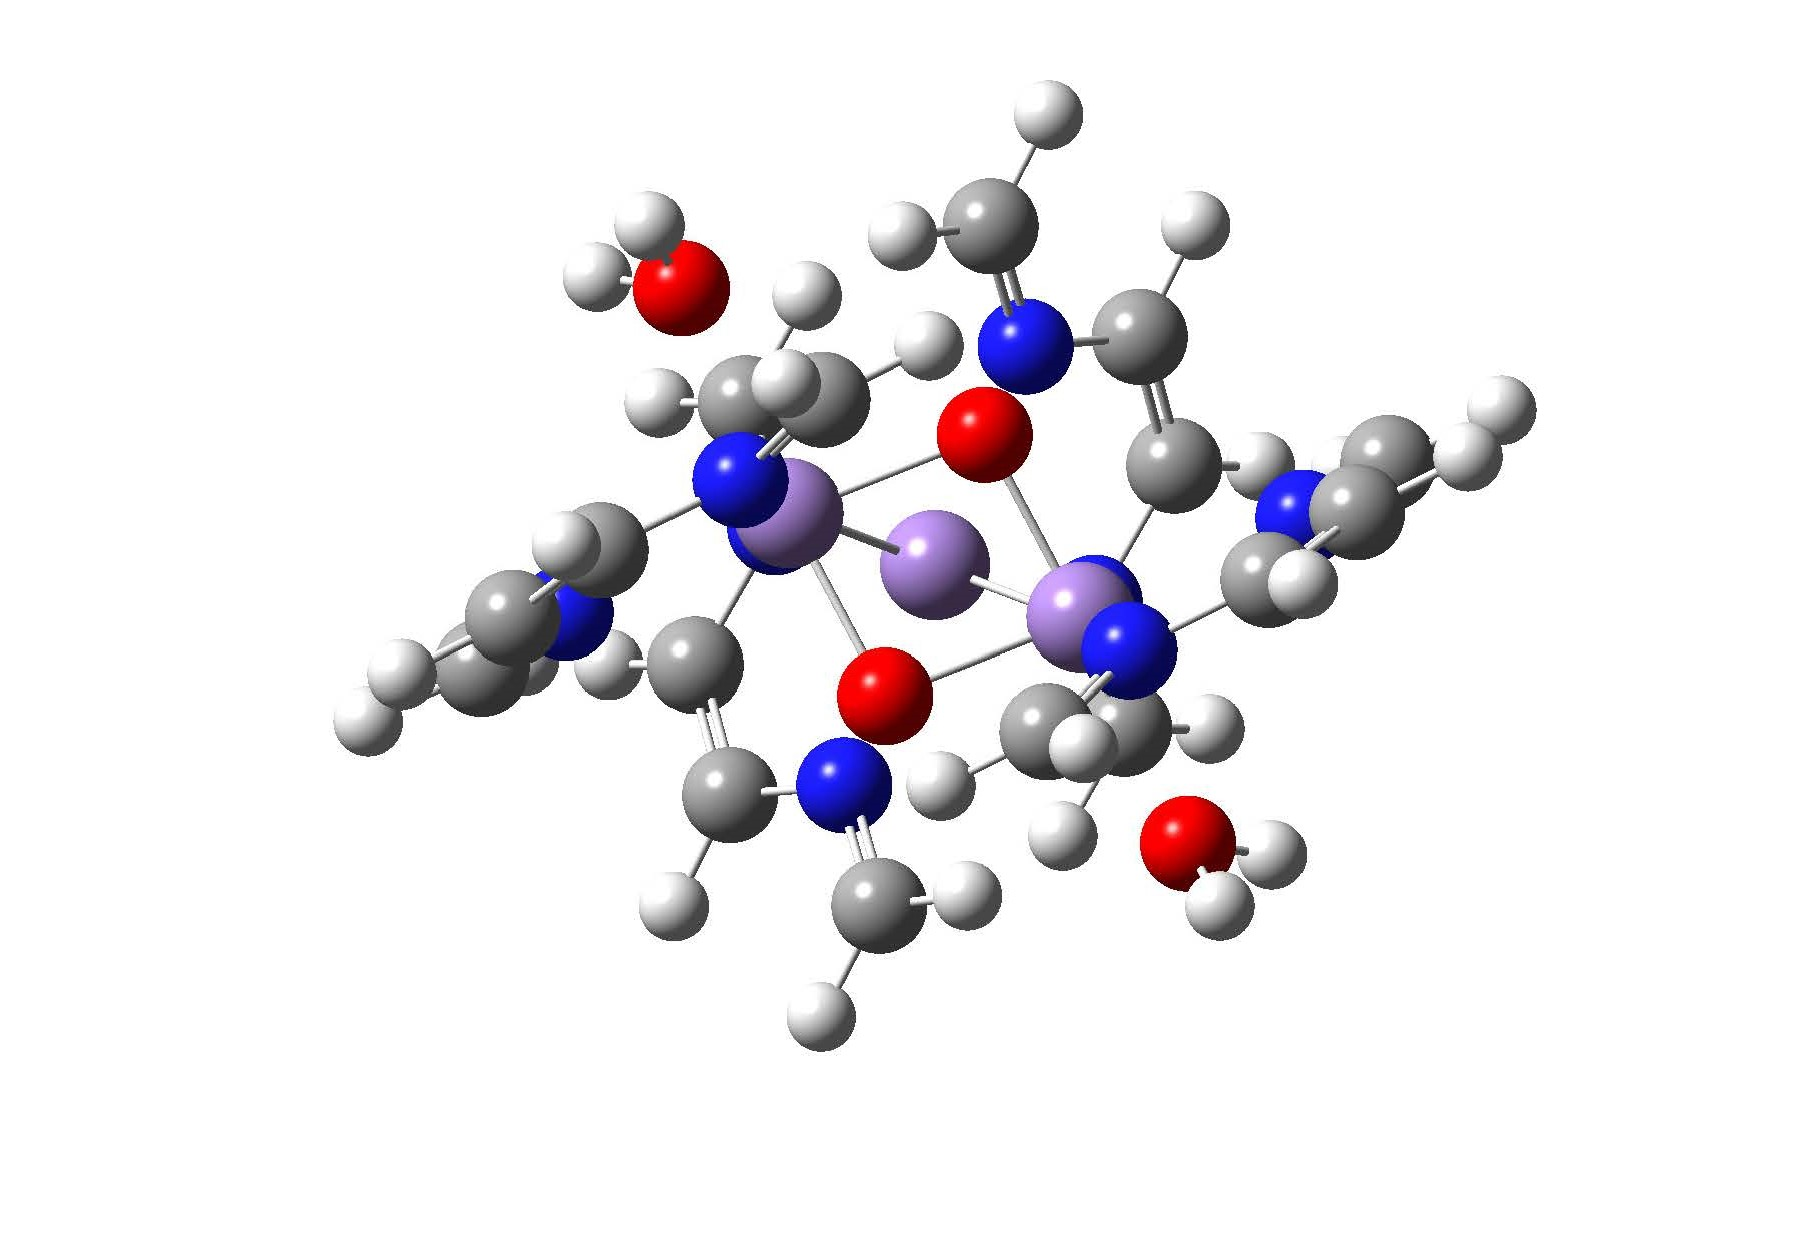
\includegraphics[width=1.0\textwidth]{figure/HF/mn32.jpg}
			Mn3配合物
		\end{figure}
		
	\end{columns}

\end{frame}


%------------------------------------------------
\begin{frame}
	\frametitle{致谢}
	感谢马海波老师的悉心指导,在论文完成的过程中给了我莫大帮助,这个课题也让我对量子化学有了更进一步的认识。\\
	感谢谢兆轩师兄与李健浩师兄在我完成论文期间,给我的一系列意见与指导,帮我解答一系列困惑。\\
	也感谢实验室其他师兄师姐在我完成毕设期间,给我提供的帮助。
\end{frame}

%------------------------------------------------

\begin{frame}
	\Huge{\centerline{谢谢!}}
	\Huge{\centerline{敬请各位老师}}
	\Huge{\centerline{批评指正!}}
\end{frame}

%----------------------------------------------------------------------------------------
\end{document} 